% BELA Chinese working manuscript. Experiments are intentionally not included.
% Compile locally with XeLaTeX and BibTeX or with an offline Tectonic bundle.
\documentclass[10pt,twocolumn,letterpaper]{article}
\usepackage[review]{cvpr}
% Chinese font support only; the supplied CVPR geometry and type sizes are unchanged.
\usepackage[UTF8,scheme=plain,fontset=fandol]{ctex}
% fontspec is loaded by ctex; restore the original CVPR Latin font families.
\renewcommand{\encodingdefault}{OT1}
\renewcommand{\rmdefault}{ptm}
\renewcommand{\sfdefault}{phv}
\renewcommand{\ttdefault}{pcr}
\ExplSyntaxOn
\cs_if_exist:NT \l__fontspec_rmfamily_encoding_tl
 {\tl_set:Nn \l__fontspec_rmfamily_encoding_tl {OT1}}
\cs_if_exist:NT \l__fontspec_sffamily_encoding_tl
 {\tl_set:Nn \l__fontspec_sffamily_encoding_tl {OT1}}
\cs_if_exist:NT \l__fontspec_ttfamily_encoding_tl
 {\tl_set:Nn \l__fontspec_ttfamily_encoding_tl {OT1}}
\ExplSyntaxOff
% Synchronize CJK heading fonts with CVPR's original 11 pt and 10 pt selectors.
\renewcommand{\elvbf}{\fontsize{11}{12}\selectfont\bfseries}
\renewcommand{\tenbf}{\fontsize{10}{12}\selectfont\bfseries}
\normalfont
%% This file contains a number of tweaks that are typically applied to the main document.
%% They are not enabled by default, but can be enabled by uncommenting the relevant lines.

%%
%% Inline annotations; for predefined colors, refer to "dvipsnames" in the xcolor package:
%% https://tinyurl.com/overleaf-colors
%%
\newcommand{\red}[1]{{\color{red}#1}}
\newcommand{\todo}[1]{{\color{red}#1}}
\newcommand{\TODO}[1]{\textbf{\color{red}[TODO: #1]}}
%%
%% disable for camera ready / submission by uncommenting these lines  
%%
% \renewcommand{\TODO}[1]{}
% \renewcommand{\todo}[1]{#1}

%%
%% work harder in optimizing text layout. Typically shrinks text by 1/6 of page, enable
%% it at the very end of the writing process, when you are just above the page limit
%%
% \usepackage{microtype}

%%
%% fine-tune paragraph spacing
%%
% \renewcommand{\paragraph}[1]{\vspace{.5em}\noindent\textbf{#1.}}

%%
%% globally adjusts space between figure and caption
%%
% \setlength{\abovecaptionskip}{.5em}


%%
%% Allows "the use of \paper to refer to the project name"
%% with automatic management of space at the end of the word
%%
% \usepackage{xspace}
% \newcommand{\paper}{ProjectName\xspace}

%%
%% Commonly used math definitions
%%
% \DeclareMathOperator*{\argmin}{arg\,min}
% \DeclareMathOperator*{\argmax}{arg\,max}

%%
%% Tigthen underline
%%
% \usepackage{soul}
% \setuldepth{foobar}
\usepackage{algorithm}
\usepackage{algorithmic}
\definecolor{cvprblue}{rgb}{0.21,0.49,0.74}
\usepackage[pagebackref,breaklinks,colorlinks,allcolors=cvprblue]{hyperref}
\def\confName{CVPR}
\def\confYear{2027}
\title{BELA：覆盖约束下的问题条件\\渐进视觉 Token 剪枝}
\author{Anonymous CVPR submission}
\begin{document}
\maketitle
\begin{abstract}
视觉语言模型把一幅图像编码成很长的 patch 序列。以 LLaVA-1.5 的常用设置为准，576 个视觉 token 进入 32 层 Decoder，既增加预填充中的注意力计算，也拉长后续解码要读取的缓存。把序列压到很小以后，选择不再只是丢掉明显背景：补进与当前问题更相关的位置，可能同时拆掉一批原本由它代表的视觉位置。本文提出 BELA。它先用视觉塔两个深度的特征做一个与问题无关的固定容量初始化，再允许问题信号对这个集合做有限次一进一出的交换；一次交换能否被接受，取决于新位置带来的问题增益，以及全体原始位置上最近代表覆盖下降了多少。被选中的仍是原模型送入投影器的特征。进入 Decoder 之后，这些 token 先参与浅层计算，再按预定层数逐段减少。在 LLaVA-1.5-7B 上，层平均保留 32 个视觉 token，对应的视觉 token-layer 预算是完整视觉序列的 $1/18$。与同一日程、同一种后层规则的原生集合相比，问题条件交换把六项任务相对完整模型的平均比值从 93.56\% 提高到 95.34\%。GQA 与 POPE F1 上升，TextVQA-OCR 下降。该比值不是答题正确率，预算比例也不是实测加速。
\end{abstract}

\section{引言}
\label{sec:intro}

视觉语言模型把视觉编码器和语言模型接到同一条生成过程里。Flamingo、BLIP-2 以及随后的 LLaVA、MiniGPT-4、InstructBLIP 说明，冻结或轻量对齐的视觉前端已经足以支持开放式图文交互~\cite{flamingo,blip2,llava,minigpt4,instructblip}。InternVL、Qwen2-VL、Qwen2.5-VL 和 LLaVA-OneVision 继续提高分辨率、增加视觉输入形式~\cite{internvl,qwen2vl,qwen25vl,onevision}。分辨率和视觉细节增加时，送入语言模型的 patch 序列通常一起变长。

主流模型用 ViT 或 CLIP 把图像切成 patch，再经投影进入 Decoder~\cite{vit,clip,llava15}。LLaVA-1.5 的常用网格是 576 个视觉 token，往往长于问题本身。对长度为 $n$、宽度为 $d$ 的序列，自注意力中的查询--键与注意力--值乘积带有 $O(n^2d)$ 项~\cite{attention}。视觉前缀因此提高预填充成本，并增加解码时要读取的 KV cache~\cite{pagedattention}。FlashAttention 降低了注意力的访存开销~\cite{flashattention,flashattention2}，前馈层、投影和缓存实现仍随序列长度变化。减少实际进入各层的视觉 token，是另一条与算子优化互补的途径。

已有工作表明，视觉序列里有大量可压缩冗余~\cite{fastv,visionzip,sparsevlm,vitcop}。VisionZip、VisPruner 和 LLaVA-PruMerge 在视觉侧挑选或合并紧凑表示，DivPrune 与 DART 分别从集合多样性和重复关系决定保留谁~\cite{visionzip,vispruner,prumerge,divprune,dart}。SparseVLM 与 PyramidDrop 则在语言模型内部按层缩减视觉序列~\cite{sparsevlm,pyramiddrop}。这些方法已经覆盖了“看视觉特征选 token”“看集合内部是否重复”和“在深层继续删”三类决策。

问题条件并没有留在这一步之外。CDPruner 用指令相关性调制 DPP 核，MMTok 用统一覆盖同时代表文本和视觉，MoB 把提示对齐与视觉保留写成带预算分配的双目标覆盖~\cite{cdpruner,mmtok,mob}。SCoRe、CoIn 和 QCPruner 进一步把显著性、信息性或问题效用放进覆盖或设施选址目标~\cite{score,coin,qcpruner}。STAR-Pro 则把入口覆盖池和后续嵌套精炼连在同一个层平均预算下~\cite{starpro}。因此，不能把“同时使用问题、覆盖和渐进剪枝”本身当作剩余问题。

仍需要单独处理的是交换的两侧并不评价同一组对象。一个位置与当前问题的相关性，描述的是它和问题代理的关系；把它换进集合时删掉的旧代表，影响的是有多少原始视觉位置失去当前最近代表。相关性高、相对已选集合也新颖的候选，仍可能拆掉一大片原先被覆盖的位置。本文研究的操作是：入口容量保持不变，问题信号只能在一个已经建好的视觉集合附近做有限次替换，而且每一次替换都要检查全体原始位置上的覆盖变化。

BELA 按这个操作组织推理。视觉塔两个深度提供选择描述，显著性最高的一部分位置作为锚点，其余名额由空间格子上的原型新颖性补足，得到与问题无关的初始集合。问题条件更新使用另一套相似度：它在同一选择描述上计算全体位置的最近代表覆盖，只接受问题增益、新颖性和覆盖下降同时满足门槛的交换，并且交换次数有硬上限。随后 Decoder 把“进入早期计算”和“继续占用后层预算”分开。第一次缩减比较当前问题响应与浅层记录的秩，第二次缩减直接按问题对视觉位置的注意力保留。送入语言模型的是原模型投影器所使用的特征，选择描述只决定索引。整个过程不更新参数。

我们在 LLaVA-1.5-7B 上固定 $64\!\rightarrow\!17\!\rightarrow\!10$ 的日程，层平均视觉 token 数为 32，视觉 token-layer 预算 $W{=}1024$。表~\ref{tab:main} 只改变入口身份。六项成绩除以固定完整模型参考后的平均值由 93.56\% 变为 95.34\%；参考值为 GQA 61.9、POPE F1 85.8、MME 1852、MMBench 64.1、ScienceQA-IMG 69.51、TextVQA-OCR 58.20。五项上升，TextVQA-OCR 由 53.41 降到 53.06。同一日程下，匹配换入数量的随机替换得到 GQA 55.96 和 POPE F1 83.34，已经高于原生集合，真实问题的更新再高于这一随机对照。把问题换成固定错配排列时 GQA 为 55.68，该对照的 POPE 没有跑完，所以问题身份目前只在 GQA 上有成对结果。POPE F1 的上升伴随召回由 73.60\% 增至 81.58\%、精度由 93.11\% 降至 91.30\%，不能写成所有幻觉类型都减少。

\begin{table}[t]
\centering
\caption{LLaVA-1.5-7B 上只改变入口身份的对照。两列共享双深度初始化、入口容量 64、事件 $11{:}17,19{:}10$ 和后层规则。GQA、ScienceQA-IMG 与 TextVQA-OCR 为准确率，POPE 为 F1，MME 为感知加认知，MMBench 为英文开发集分数。末行是六项相对固定完整模型参考的算术平均。}
\label{tab:main}
\small
\setlength{\tabcolsep}{4pt}
\begin{tabular}{lcc}
\hline
任务 & 原生集合 & 问题条件更新 \\
\hline
GQA & 55.57 & 56.52 \\
POPE F1 & 82.21 & 86.16 \\
MME & 1651.78 & 1715.68 \\
MMBench-EN & 61.34 & 61.77 \\
ScienceQA-IMG & 68.91 & 69.61 \\
TextVQA-OCR & 53.41 & 53.06 \\
\hline
六任务归一化平均 & 93.56\% & 95.34\% \\
\hline
\end{tabular}
\end{table}

本文的贡献有三点。第一，把严格入口预算下的问题适配定义成对已有视觉集合的有限交换，并区分初始化所用的空间原型规则和更新所用的群体覆盖。第二，给出由问题增益、新颖性和覆盖变化共同筛选的同容量交换，以及移除损失与加入补偿的分解和累计变化范围。第三，把该集合接到固定的 Decoder 日程上：第一次精炼使用问题响应的秩漂移，第二次使用问题注意力，并在上述同日程对照中报告入口身份变化的效果与文字任务上的下降。

\section{相关工作}
\label{sec:related}

\paragraph{视觉侧的紧凑输入。}
DynamicViT、A-ViT、EViT 和 ATS 在视觉 Transformer 内部按输入或注意力减少 token，ToMe 合并相近 token，TokenLearner 学习紧凑表示~\cite{dynamicvit,avit,evit,ats,tome,tokenlearner}。进入视觉语言模型之后，VisionZip 区分主导内容与上下文并改写保留表示，LLaVA-PruMerge 在采样之外补充被丢掉的信息，VisPruner 结合视觉重要性与去重~\cite{visionzip,prumerge,vispruner}。DivPrune 把保留集合写成最大最小多样性问题，DART 用随机对照说明重复关系可以比单独的重要性排序更决定结果~\cite{divprune,dart}。BELA 也在语言模型之前把 576 个位置收成固定入口，但送入 Decoder 的仍是被选中位置上的原始投影特征，不合并 hidden state。入口处的新颖性只用于提出候选和计算空间原型，不能代替后文对全体位置覆盖变化的检查。

\paragraph{问题条件的集合目标。}
CDPruner 把问题相关性写进 DPP 核，使子集概率偏向与指令相关且彼此多样的 token~\cite{cdpruner}。MMTok 以平均最大相似度定义覆盖，校准后联合文本目标与视觉目标，再贪心构造集合~\cite{mmtok}。MoB 在几何假设下分析视觉保留和提示对齐的耦合，并把预算分给两个目标~\cite{mob}。SCoRe 用显著性加权的 $k$-center 组织代表性，CoIn 把信息性与基于体积的集合选择合在一起，QCPruner 的设施选址增益则同时用问题效用加权视觉目标和候选代表~\cite{score,coin,qcpruner}。这些工作优化的是一次性的集合目标。BELA 的更新从已经选定的 $K$ 个索引出发，每次只替换一个成员，可行域同时限制问题增量、相对当前集合的新颖性和覆盖下降，总替换次数另有上限。问题分数决定交换方向，不作为群体两侧的同一权重。更新阶段的平均最近代表相似度也没有被初始化最大化，因此不能套用次模贪心的近似界~\cite{linbilmes2011}。

\paragraph{深度、日程与渐进删除。}
FastV 利用浅层语言模型中的注意力做一次性剪枝，PyramidDrop 先比较不同层位和删减比例，再把保留数量排成逐段日程~\cite{fastv,pyramiddrop}。SparseVLM 用文本评分者调节比例并回收 token；其所讨论的实现包含与高效注意力兼容的路径，本文不把它概括成一律无法使用 FlashAttention~\cite{sparsevlm}。FitPrune 用注意力分布拟合预算内的剪枝方案，VFlowOpt 把重要性、回收和信息流引导的策略搜索接在一起~\cite{fitprune,vflowopt}。ViTCoP 把视觉端筛选、浅层协同和深层精剪分成不同阶段，AgilePruner 与 AutoSelect 则分别从行为分析和可训练噪声门控研究选择依据~\cite{vitcop,agilepruner,autoselect}。HiPrune 比较视觉深度上的注意力，ATP-LLaVA 学习样本和层相关的阈值~\cite{hiprune,atpllava}。

更近的工作已经把覆盖和渐进执行放在一起。STAR-Pro 使用前端特征覆盖池和嵌套的层间精炼，并报告层平均预算~\cite{starpro}。CoRePrune 说明一个 token 能否删除依赖于深度和当时的集合，Hi-Lo Prune 在删除前把信息转到保留表示里~\cite{coreprune,hiloprune}。BELA 沿用固定的分段数量，不把日程形状当作新的原理。本文相对这些工作的具体差别是入口处的受约束交换，以及第~\ref{sec:progressive} 节写出的两段后层规则：第一剪点用问题响应的秩漂移重排，第二剪点用问题注意力，二者都保持当前存活集合的嵌套。

\section{方法}
\label{sec:method}

\subsection{预算、索引与实际送入模型的特征}
\label{sec:overview}

给定图像和问题，视觉塔产生 $N$ 个与原始 patch 对齐的位置。LLaVA-1.5 使用 CLIP-ViT-L/14-336，网格为 $24\times 24$，故 $N{=}576$，语言模型有 $L{=}32$ 层~\cite{llava15,clip}。记第 $\ell$ 个 Decoder block 实际处理的视觉 token 数为 $K_\ell$。视觉 token-layer 预算、层平均数量和相对完整视觉序列的比例分别是
\begin{equation}
 W=\sum_{\ell=1}^{L}K_\ell,\qquad
 \bar K=W/L,\qquad
 \rho_W=W/(LN).
 \label{eq:budget}
\end{equation}
$W$ 只累计各层看见的视觉 token 个数。它不包含文本长度，也不等于 FLOPs、延迟或显存。

选择发生在两个地方，如图~\ref{fig:framework}。语言模型之前，方法确定入口集合 $S$，且 $|S|{=}K_0$。语言模型内部，指定 block 结束后把当前存活集合嵌套地收成更小的集合。两条路径使用的特征不同。选择描述只参与比较位置；真正进入投影器和 Decoder 的，是视觉塔倒数第二个 block 的 patch 特征按索引取出的那些行。代码在选择前检查这些行与投影器输入逐元素一致。被删位置不再出现在后续 block 的隐藏状态里，其 RoPE 位置编号保持删除前的原始编号，不重新排成连续整数。

\begin{figure*}[t]
 \centering
 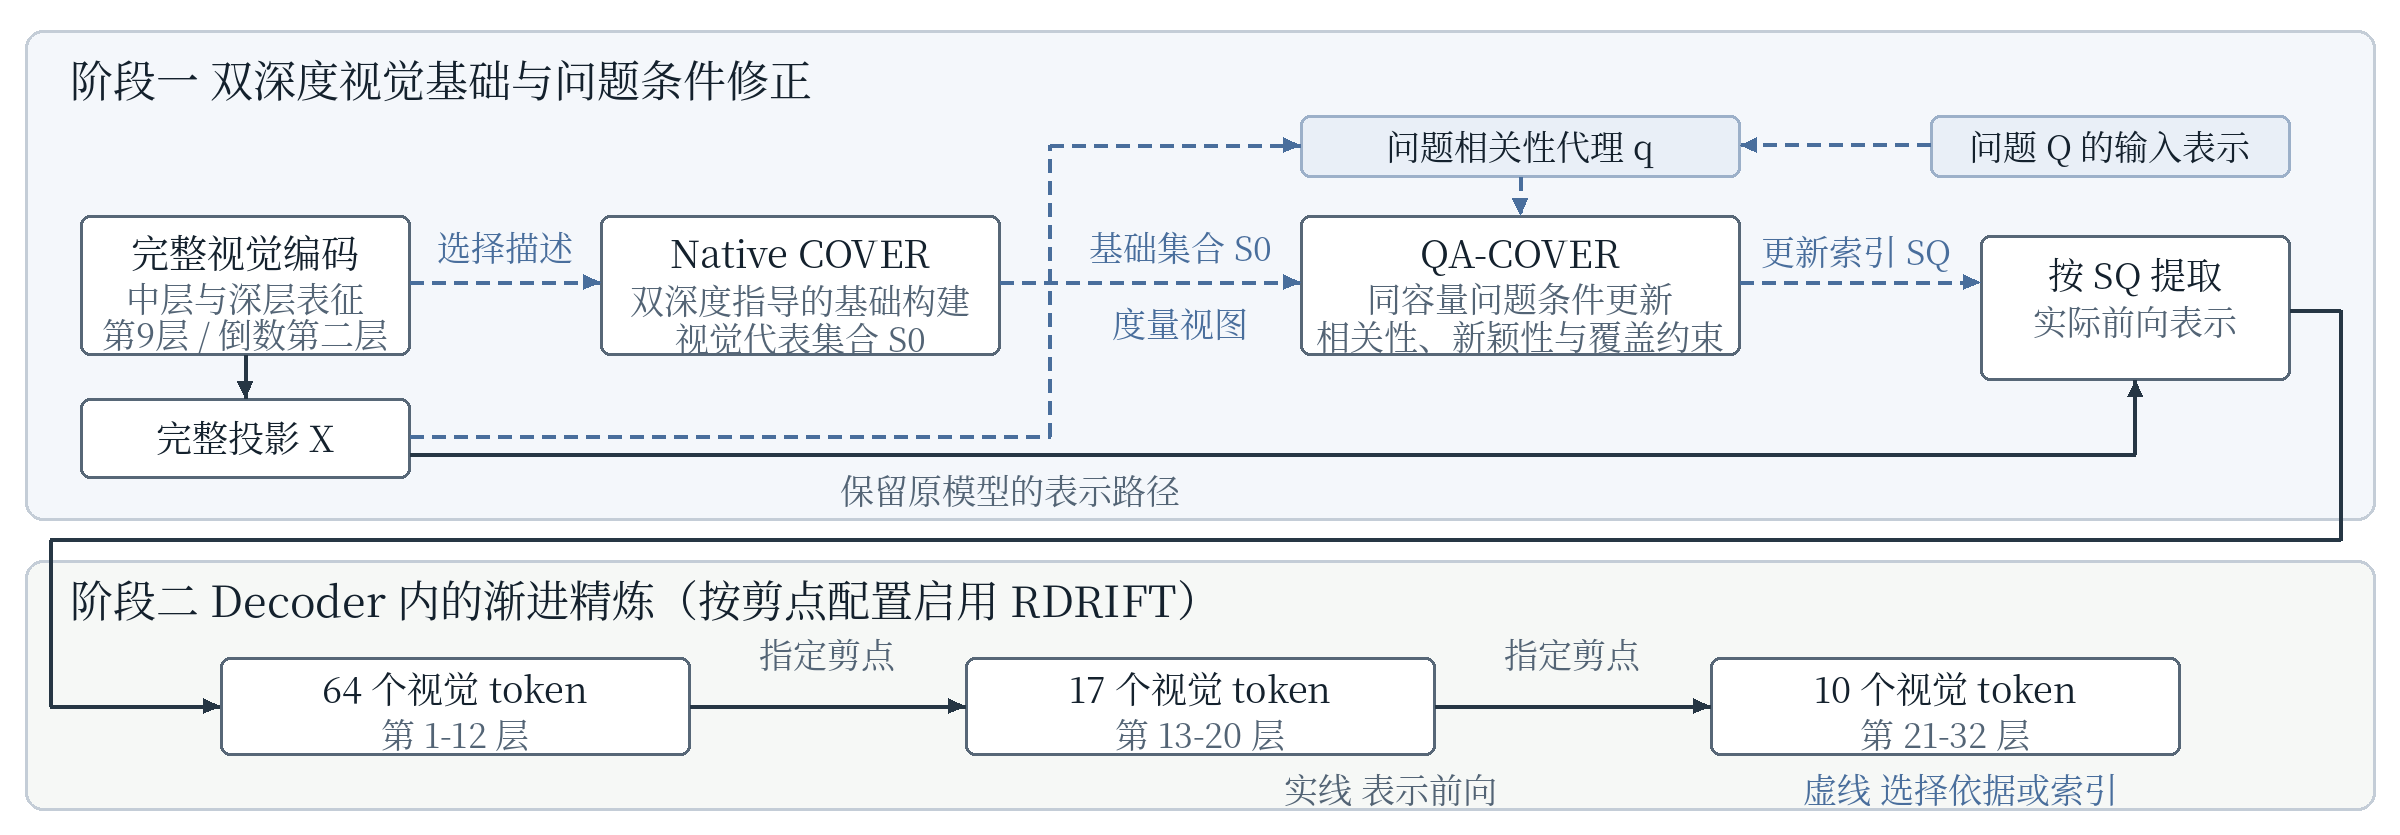
\includegraphics[width=\textwidth]{figures/bela_framework.png}
 \caption{BELA 的两条路径。虚线是选择描述或索引，实线是进入投影器与 Decoder 的原始特征。初始化用双深度显著性与 $4\times 4$ 空间原型补足锚点；问题条件更新在另一套全体位置覆盖上做有限次交换。图中层号从 1 计：第 1--12、13--20、21--32 层分别对应正文从 0 计的 block 0--11、12--19、20--31。图中的秩漂移只用于第一次剪枝；第二次剪枝使用问题注意力。$64\!\rightarrow\!17\!\rightarrow\!10$ 是 $W{=}1024$ 的数量日程。}
 \label{fig:framework}
\end{figure*}

\subsection{双深度描述与空间原型初始化}
\label{sec:visualbase}

记 CLIP 的 hidden state 包含嵌入输出。第 9 个 Transformer block 的 patch 输出记为 $F^{(9)}$，对应 \texttt{hidden\_states[9]}，其 CLS 到 patch 的注意力取 \texttt{attentions[8]}。倒数第二个 block 的 patch 输出记为 $F^{\mathrm{pen}}$，对应 \texttt{hidden\_states[-2]} 与 \texttt{attentions[-2]}。两层的第 $i$ 行都是同一个原始 patch。显著性是多头注意力中 CLS 对 patch 的和，不是先对头取平均再做 $\ell_1$：
\begin{equation}
 s^{(9)}_i=\sum_{h}A^{(9)}_{h,0,i},\qquad
 s^{\mathrm{pen}}_i=\sum_{h}A^{\mathrm{pen}}_{h,0,i}.
\end{equation}
报告配置取 $\beta{=}0.5$，融合分数与选择描述为
\begin{equation}
\begin{aligned}
 s_i&=(1-\beta)s^{\mathrm{pen}}_i+\beta s^{(9)}_i,\\
 z_i&=\big[\sqrt{1-\beta}\,\hat u(F^{\mathrm{pen}}_i);\;
           \sqrt{\beta}\,\hat u(F^{(9)}_i)\big].
\end{aligned}
\label{eq:dual}
\end{equation}
$\hat u$ 表示按通道做 $\ell_2$ 归一化，稳定项为 $10^{-12}$。$z_i$ 是两层宽度的拼接。对 CLIP-ViT-L，单层宽度为 1024，拼接后为 2048。这个描述用于选索引，不替换 $F^{\mathrm{pen}}$。

初始化调用既有的 REPLACE/COVER 规则，入口 $K_0{=}64$，替换名额 $b{=}32$。锚点是融合显著性最高的 $K_0-b{=}32$ 个位置。候选池不是锚点之外的全部位置，而是融合显著性前 $K_0$ 名之外的 $N-K_0$ 个位置；因此显著性排名第 33 到第 64 的位置既不是锚点，也不会被补入。把 $24\times 24$ 网格划成 $4\times 4$ 个格子，每格 $6\times 6$。令 $\hat z_i$ 为对 $z_i$ 再次归一化的结果，稳定项为 $10^{-8}$。格子 $g$ 的原型是落在该格中的锚点特征的均值，然后再归一化；空格子的原型为零向量。位置 $i$ 的效用是
\begin{equation}
 u_i=s_i\Big(1-\operatorname{clip}\big(\cos(\hat z_i,m_{g(i)}),0,1\big)\Big).
 \label{eq:native}
\end{equation}
空格子的原型是零向量，余弦为零，效用退化为显著性本身。初始集合 $S_0$ 由 32 个锚点和效用最高的 32 个池外位置组成，再按原始 patch 编号排序。这一步只执行一次，不迭代最大化下一节的覆盖函数 $C$。它与问题无关。

\subsection{问题条件的同容量交换}
\label{sec:queryupdate}

更新从 $S_0$ 出发，容量始终为 $K_0$。报告配置把显著性保护名额设为 0，因此交换阶段不再用 CLS 分数保护任何成员。问题代理与外部预计算分数二选一；本文的运行使用嵌入路径。先用已有的多模态投影器处理全部 $N$ 个 $F^{\mathrm{pen}}$ 行，得到与语言模型同宽的向量 $x_i$。问题 token 去掉模板词和标点，只保留内容片段；若内容片段为空，或原始分数的总体标准差低于 $0.008$，则保持 $S_0$ 不变。设内容片段的输入嵌入为 $\{e_t\}$，
\begin{equation}
\begin{gathered}
 \bar e=\frac{1}{|Q_c|}\sum_{t\in Q_c}e_t,\qquad
 a_i=\cos(x_i,\bar e),\\
 q_i=\sigma\Big(\operatorname{clip}\big(\frac{a_i-\operatorname{med}(a)}{2\,\operatorname{std}(a)},-8,8\big)\Big).
\end{gathered}
\label{eq:query}
\end{equation}
$\sigma$ 是 sigmoid，$\operatorname{clip}$ 把数值截到给定区间。标准差是总体标准差，分母的下限为 $10^{-12}$。偶数长度时中位数取排序后两个中间值中较低的一个。$q_i$ 是问题方向的代理，不是经过专门对齐训练的相关性概率。

覆盖使用式~\eqref{eq:dual} 的描述，并且只传入这一个视图。对每一行再次做 $\ell_2$ 归一化后，
\begin{equation}
\begin{aligned}
 G_{ij}&=\operatorname{clip}\big(\cos(z_i,z_j),0,1\big),\\
 C(S)&=\frac1N\sum_{i=1}^{N}\max_{j\in S}G_{ij},\\
 \nu(v\mid S)&=1-\max_{j\in S}G_{vj},\quad v\notin S.
\end{aligned}
\label{eq:coverage}
\end{equation}
$C(S)$ 是全体原始位置到当前集合的平均最近代表相似度。$\nu$ 只比较候选和当前集合，二者不是同一个量。$G$ 由截断余弦得到，不假设它是度量，也不把 $1-C(S)$ 解释成率失真。

每一轮都按当前集合重新排序候选，先前被移出的位置可以再次进入。集合外位置按 $q_v\nu(v\mid S)$ 取前 $P_a{=}16$ 个；集合内位置按
\begin{equation}
 p_{\mathrm{drop}}(u)=1-q_u+\frac12\max_{j\in S,\,j\neq u}G_{uj}
 \label{eq:drop}
\end{equation}
取前 $P_d{=}12$ 个。单元素集合的内部冗余取零。对一对 $(u,v)$，令 $S'=(S\setminus\{u\})\cup\{v\}$，$\Delta q=q_v-q_u$，$\Delta C=C(S')-C(S)$。可行条件为
\begin{equation}
 \Delta q\ge \gamma,\qquad
 \nu(v\mid S)\ge \tau_\nu,\qquad
 \Delta C\ge -\varepsilon,
 \label{eq:feasible}
\end{equation}
报告配置中 $\gamma{=}0.08$、$\tau_\nu{=}0.05$、$\varepsilon{=}0.005$。在可行对中最大化
\begin{equation}
 J(u,v)=\Delta q\,\nu(v\mid S)+\lambda\Delta C,
 \label{eq:swap}
\end{equation}
$\lambda{=}0.5$。实现取可行分数中的最大有限值，没有额外的 $J>0$ 判断。没有可行对，或已完成 $B{=}8$ 次交换时停止。$B$ 是上限，不保证每次样本都交换满 8 次。接受后按原始编号排序，得到 $S_Q$。

匹配随机对照保留同一次运行实际删除的位置和相同的净交换数，只把新增位置换成种子为 17 的随机位置。错配对照仍走式~\eqref{eq:query}--\eqref{eq:swap}，但问题向量来自固定的错配排列。

\subsection{移除损失与变化范围}
\label{sec:mechanism}

设 $R=S\setminus\{u\}$，空集的最大相似度为 0，并记 $b_i(R)=\max_{j\in R}G_{ij}$。一次交换的覆盖变化可以拆开：
\begin{equation}
\begin{aligned}
 D_C(u\mid S)&=C(S)-C(R)
  =\frac1N\sum_{i=1}^{N}[G_{iu}-b_i(R)]_+,\\
 A_C(v\mid R)&=\frac1N\sum_{i=1}^{N}[G_{iv}-b_i(R)]_+,\\
 \Delta C&=A_C(v\mid R)-D_C(u\mid S).
\end{aligned}
\label{eq:decomposition}
\end{equation}
$D_C$ 是 $u$ 对全体位置的不可替代程度，不等于 $1-q_u$。$A_C$ 是 $v$ 能把多少位置的最近代表提高，不等于 $\nu(v\mid S)$。式~\eqref{eq:feasible} 的覆盖门因此等价于加入补偿至少补上移除损失超出 $\varepsilon$ 的部分。

一个构造例子可以分开这两个量，它不是实验样本。100 个位置分成 50、49、1 的三簇，簇内相似度为 1，簇间为 0。保留前两簇各一个代表时 $C{=}0.99$。若用第三簇的唯一点替换第一簇的代表，该点相对当前集合的新颖性为 1，但覆盖降到 0.50：移除损失 0.50，加入补偿 0.01。高新颖性仍可能破坏大量已有代表关系。反过来，若答案恰好落在被拒绝的小簇里，平均覆盖约束也会留下它。所以 $C$ 保护的是特征代理下的代表关系，不是答案充分性。

设实际接受 $T\le B$ 次交换。一进一出和逐步门槛给出
\begin{equation}
\begin{gathered}
 |S_Q|=K_0,\qquad |S_Q\cap S_0|\ge K_0-T,\\
 C(S_Q)\ge C(S_0)-T\varepsilon,\\
 \sum_{i\in S_Q}q_i\ge \sum_{i\in S_0}q_i+T\gamma .
\end{gathered}
\label{eq:bounds}
\end{equation}
$K_0{=}64$、$T\le 8$ 时，最终集合至少还留着 56 个初始身份，累计覆盖下降不超过 $0.04$。这是式~\eqref{eq:coverage} 上的范围。可行对还满足 $J\ge \gamma\tau_\nu-\lambda\varepsilon=0.0015$，该下界来自门槛，不是实现里另写的判断。$J$ 依赖当前集合，算法没有在优化一个固定的全局目标，也没有次模近似保证。

\subsection{Decoder 内的两次精炼}
\label{sec:progressive}

$S_Q$ 对应的 $F^{\mathrm{pen}}$ 行与文本一起进入 Decoder。报告日程的段长是 12、8、12 层，保留数量是 64、17、10。实现在第 11 和 第 19 个 block（从 0 计数）结束后剪枝，事件写成 $11{:}17,19{:}10$。于是第 0--11 个 block 处理 64 个视觉 token，第 12--19 个处理 17 个，第 20--31 个处理 10 个：
\begin{equation}
 W=64\times 12+17\times 8+10\times 12=1024.
 \label{eq:schedule}
\end{equation}
因而 $\bar K{=}32$，$\rho_W{=}1/18\approx 5.56\%$，相对完整视觉序列少 $17/18\approx 94.44\%$。两次剪枝都从当前仍在序列中的视觉位置里选择，后一层的保留集合是前一层的子集。

两次使用的分数不同。第 0 个 block 之后，把问题到视觉的注意力行按问题 token 的原有顺序切成至多 4 段连续桶，保存每桶的平均。注意力本身先在完整合法前缀上做 softmax，再对头取平均，最后只留下视觉列。第一次剪枝时，用原始 patch 编号把这份浅层记录对齐到当前 64 个位置。令 $\bar\rho^{\mathrm{now}}$ 与 $\bar\rho^{\mathrm{old}}$ 分别为当前响应和浅层响应在桶上的平均。秩函数 $\pi$ 对向量做稳定的升序排序，最小值为 0、最大值为 1，并列项按原有顺序占据相邻秩，除以 $n-1$，不把并列项改成平均秩。第一次剪枝的分数是
\begin{equation}
 r_i=w\,\pi(\bar\rho^{\mathrm{now}})_i
 +(1-w)\big(\pi(\bar\rho^{\mathrm{now}})_i-\pi(\bar\rho^{\mathrm{old}})_i\big),
 \label{eq:rdrift}
\end{equation}
报告配置 $w{=}0.6$。保留 $r_i$ 最高的 17 个位置。这个排序直接决定第一次剪枝，不再使用该层的问题注意力 Top-$K$。第二次剪枝不读取式~\eqref{eq:rdrift}。它把问题位置上的视觉列注意力对问题 token 取平均，保留最高的 10 个。

隐藏状态在剪枝时按保留行聚集。报告运行的缓存策略是逐层局部缓存：已经执行过的 block 不回溯删除自己的 KV。因此前 12 层的缓存仍对应 64 个视觉位置，中间 8 层对应 17 个，最后 12 层对应 10 个。解码时，新 token 在浅层仍能读到入口集合的键值，在深层只能读到当时留下的视觉位置。末层存活数量不能代表全部缓存。一个入口位置后来被删掉，只说明它没有进入最后 12 层的隐藏状态，不能由此推出它的信息已经被文本状态吸收。

\subsection{执行过程与实际计算}
\label{sec:cost}

算法~\ref{alg:bela} 汇总上述顺序。视觉塔对全部 patch 做一次前向。问题代理额外调用一次全网格投影器，这 576 次投影不属于原生集合那一支的成本。式~\eqref{eq:coverage} 的相似度是 $N\times N$，描述宽度为两层通道数之和。每轮交换复用当前集合的最大和次大相似度，主要计算量随 $NK_0+NP_aP_d$ 增长。剪点上为了得到问题响应，实现会由该层的查询和键显式形成问题位置的 logits；报告运行的注意力后端是 SDPA，这几层的选择统计不能算成已被注意力内核完全吸收。

\begin{algorithm}[t]
\caption{BELA 的一次推理}
\label{alg:bela}
\begin{algorithmic}[1]
\REQUIRE 图像，问题，入口容量 $K_0$，段长与保留数
\STATE 视觉编码，取 $F^{(9)}$、$F^{\mathrm{pen}}$ 与 CLS 和显著性
\STATE 按式~\eqref{eq:dual}、\eqref{eq:native} 得到 $S_0$
\STATE $S\leftarrow S_0$；用全网格投影和内容嵌入算 $q$
\IF{$\operatorname{std}(q)\ge 0.008$}
 \STATE 由 $z$ 构造 $G$
 \FOR{$t=1,\ldots,\min(B,K_0,N-K_0)$}
  \STATE 按当前 $S$ 取加入池与移除池
  \IF{没有满足式~\eqref{eq:feasible} 的交换}
   \STATE \textbf{break}
  \ENDIF
  \STATE 按式~\eqref{eq:swap} 替换一对并重排 $S$
 \ENDFOR
\ENDIF
\STATE 以 $F^{\mathrm{pen}}_{S}$ 与文本进入 Decoder
\STATE block 11 后按式~\eqref{eq:rdrift} 留 17 个
\STATE block 19 后按问题注意力留 10 个
\STATE 聚集后续隐藏状态与位置编号
\STATE 已完成层的 KV 保持该层当时的长度
\ENSURE 各层视觉数量满足式~\eqref{eq:schedule}
\end{algorithmic}
\end{algorithm}

设第 $\ell$ 层序列长度为 $n_\ell=K_\ell+L_t$，$L_t$ 为文本长度，$d$ 与 $d_{\mathrm{ff}}$ 为隐藏宽度和前馈宽度。语言模型主体的计算规模是
\begin{equation}
 O\Big(\sum_{\ell=1}^{L}(n_\ell d^{2}+n_\ell^{2}d+n_\ell\,d\,d_{\mathrm{ff}})\Big).
 \label{eq:llmcost}
\end{equation}
式~\eqref{eq:budget} 只解释其中视觉 token 的个数。完整成本还要加上视觉塔、全网格投影、相似度、剪点上的问题--键乘积，以及解码时长短不一的缓存读取~\cite{flashattention,flashattention2,pagedattention}。

% % Intentionally excluded from this revision, as requested by the authors.
% Populate and enable the input in main.tex after the experimental section is ready.

\section{结论}
\label{sec:conclusion}

本文把严格入口预算下的问题适配写成对一个已有视觉集合的有限更新。BELA 用两个视觉深度上的显著性与空间原型新颖性确定初始身份，再用问题嵌入代理提出交换，并用全体视觉位置的最近代表覆盖变化决定这次交换能否发生。进入 Decoder 后，第一次缩减按问题响应相对浅层记录的秩漂移排序，第二次缩减按问题到视觉的注意力保留。初始化与更新使用不同的集合函数，它们通过被传递的索引集合连接，而不是对同一个目标做两轮求解。

在 LLaVA-1.5-7B、$W{=}1024$ 的固定日程上，这一入口更新提高了六任务归一化平均，并在 GQA 与 POPE 上超过匹配换入数量的随机替换；错配问题在已完成的 GQA 上弱于真实问题。TextVQA-OCR 同时下降。覆盖约束限制的是特征代理上的代表关系，不保证答案证据被保住。视觉塔仍然完整执行，全网格投影、成对相似度和剪点上的问题--键乘积都会计入实际成本；各层缓存长度等于该层真正处理过的序列，不能按末层 10 个 token 统一估计。本文没有把上述数量预算写成延迟或显存收益。

\section*{LLM Usage Statement}
本研究使用大型语言模型辅助文献整理、方法讨论、中文稿起草和编译检查。
作者核对了最终稿中的算法定义、实现路径、引用语境和实验记录，并对论文中的科学结论承担责任。

{\small
\bibliographystyle{ieeenat_fullname}
\bibliography{references}
}
\end{document}
